\documentclass{article}

\usepackage[utf8]{inputenc} 

\usepackage[table]{xcolor}
\usepackage{graphicx}
\usepackage{microtype}
\usepackage{hyperref}
\hypersetup{
    colorlinks=true,
    linkcolor=blue,
    filecolor=magenta,      
    urlcolor=blue,
}

\usepackage{wasysym}  % Emoji

\setlength{\parskip}{0.15cm}  % increase skip on paragraphs

% Section number
\setcounter{secnumdepth}{0}  % Do not number any sections. This breaks referencing
\usepackage{nameref}         % Use referencing by name if no section numbers are used

\usepackage{longtable}
\usepackage{makecell}


\usepackage[letterpaper, textwidth=160mm, textheight=240mm, bindingoffset=1cm]{geometry}

\usepackage{calc}
\newlength{\lmargin}
\setlength{\lmargin}{1in + \hoffset + \oddsidemargin}

\usepackage{flowfram}

\usepackage{color}
\usepackage{colortbl}

\usepackage{tikz}


\newflowframe[1]{7.5cm}{27\baselineskip}{0cm}{0\baselineskip}[frame1-1a]
\vspace{0.5cm}
\newflowframe[1]{7.5cm}{27\baselineskip}{8.5cm}{0\baselineskip}[frame1-2b]
%\newflowframe[1]{5cm}{27\baselineskip}{11cm}{0\baselineskip}[frame1-3c]

\newstaticframe[1]{\paperwidth}{14cm}{-\lmargin}{12.5cm}[frameS-1a]
\newstaticframe[1]{14cm}{7\baselineskip}{0cm}{45\baselineskip}[frameS-1b]

\newdynamicframe[odd]{2cm}{2cm}{-\lmargin}{6cm}[frameD-1a]
\newdynamicframe[even]{2cm}{2cm}{\textwidth+\lmargin-3cm}{6cm}[frameD-1b]

\newstaticframe[2]{\paperwidth}{14cm}{-\lmargin}{12.5cm}[frameS-2a]
\newflowframe[2]{15.5cm}{27\baselineskip}{0cm}{0\baselineskip}[frame2-1b]
\newflowframe[>2]{15.5cm}{57\baselineskip}{0cm}{0\baselineskip}[frame3-1a]
%\newflowframe[>1]{7.5cm}{57\baselineskip}{8.5cm}{0\baselineskip}[frame2-2a]
%\newflowframe[>1]{5cm}{57\baselineskip}{11cm}{0\baselineskip}[frame2-3a]

\definecolor{blue}{rgb}{0.13, 0.3, 0.55}


\begin{document}

\pagestyle{empty}

\begin{dynamiccontents*}{frameD-1a}
\begin{tikzpicture}
\draw(0,0) node [fill=blue, minimum width=2cm, minimum height=2cm]{
{\sffamily\bfseries\Huge\color{white}\thepage}
};
\end{tikzpicture}
\end{dynamiccontents*}

\begin{dynamiccontents*}{frameD-1b}
\begin{tikzpicture}
\draw(0,0) node [fill=blue, minimum width=2cm, minimum height=2cm]{
{\sffamily\bfseries\Huge\color{white}\thepage}
};
\end{tikzpicture}
\end{dynamiccontents*}


\begin{staticcontents*}{frameS-1a}

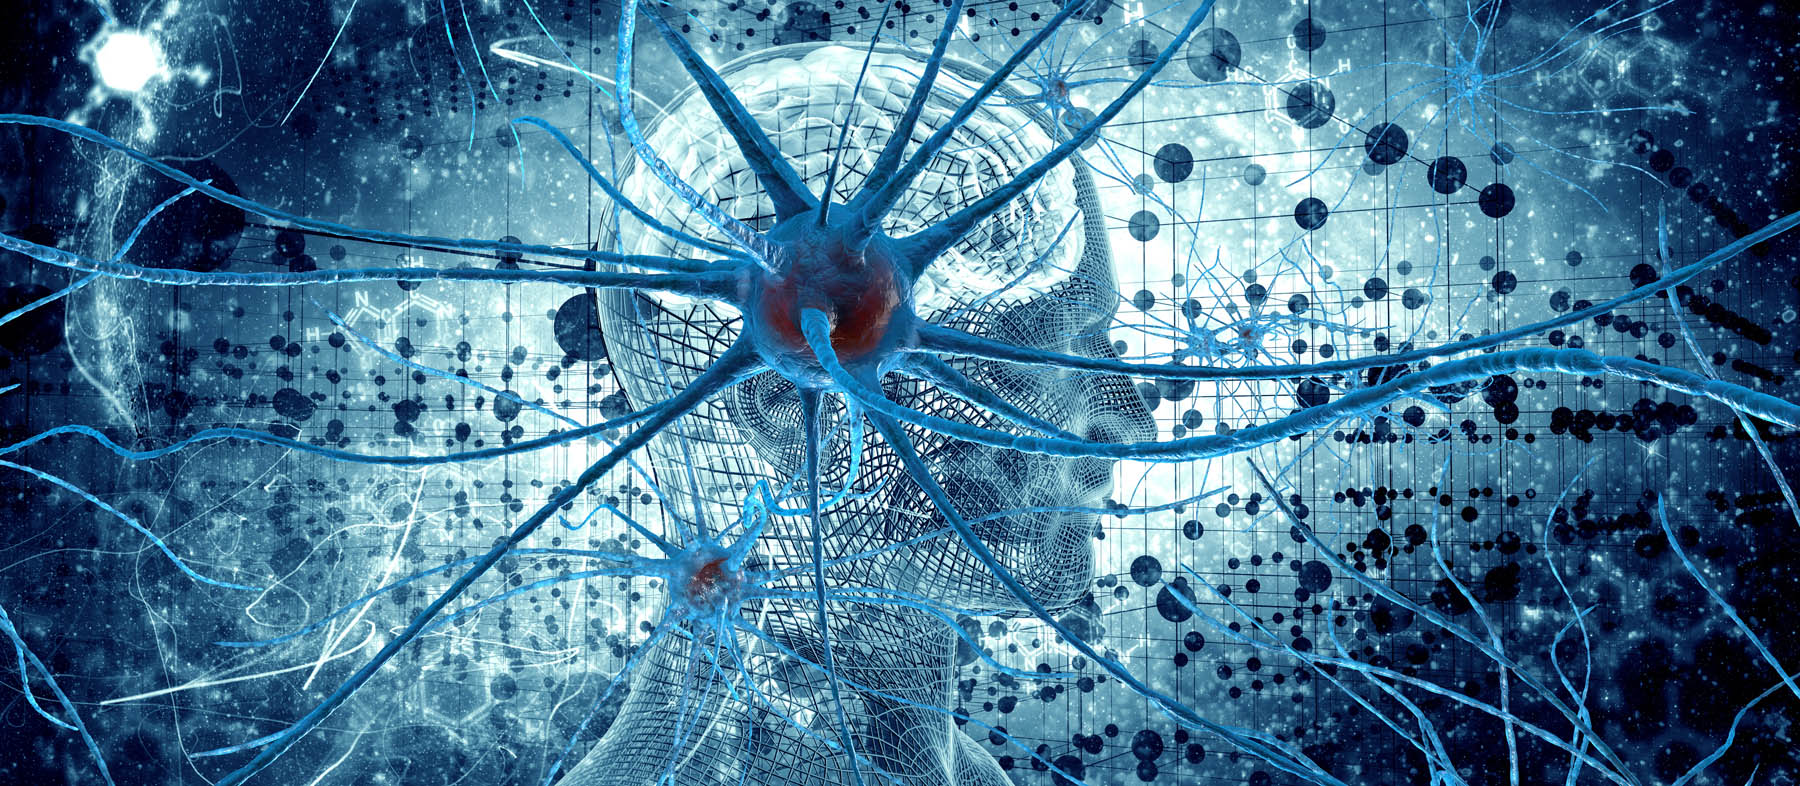
\includegraphics[width=\textwidth]{nwb-neurophysiology.jpg}
\small \textit{Image courtesy of \href{https://www.nwb.org/}{www.nwb.org}}
\end{staticcontents*}


\begin{staticcontents*}{frameS-1b}
\vspace{1.8cm}
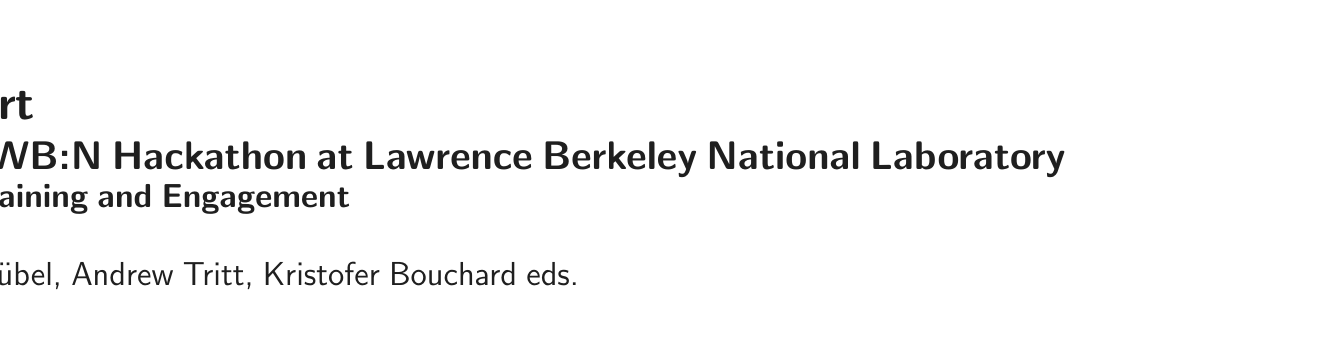
\begin{tikzpicture}
\draw(0,0) node [fill=white, text width=15cm, inner sep=6mm, opacity=0.88]{
\large\sffamily 
\LARGE\textbf{Report}\\
\Large\textbf{5th NWB:N Hackathon at Lawrence Berkeley National Laboratory} \\
\large\textbf{User Training and Engagement} \\ 
\vspace{0.5cm}
\large Oliver R\"ubel, Andrew Tritt, Kristofer Bouchard eds. \\
\vspace{0.5cm}
};
\end{tikzpicture}
\end{staticcontents*}

\small

\section*{Participants}

\begin{itemize}
\setlength\itemsep{0cm}
\item Oliver Ruebel	(LBNL)
\item Andrew Tritt	(LBNL)
\item Kristofer Bouchard (LBNL, NSE Lab)
\item Max Dougherty (LBNL, NSE Lab)
\item Tom Davidson (UCSF - Frank Lab)
\item Karen Lavi (UCSF)
\item Ali Mohebi	(UCSF)
\item Dylan Paiton (UCB)
\item Evan Lyall (UCB)
\item Jeff Teeters (UCB)
\item Stephanie Albin (The Kavli Foundation)
\item Kevin Brown (New York University)
\item David Tingley (NYU)
\item Sam McKenzie (NYUMC)
\item Sebi Rolotti	(Columbia University, Losonczy Lab)
\item Jochen Weber (Columbia University, Zuckerman Mind Brain Behavior Institute)
\item David Thibodeaux (Columbia University)
\item Ben Dichter	(Stanford)
\item Aaron Milstein (Stanford University)
\item Ivan Raikov	(Stanford University)
\item Kei Masuda (Stanford University, Giocomo Lab)
\item Jason Bant (Stanford University)
\item Adam Granger (Harvard Medical School)
\item Duo Xu (Johns Hopkins University)
\item Eric Finkel (Johns Hopkins School of Medicine, O’Connor Lab)
\item Michael Grauer (Kitware)
\item Jean-Christophe Fillion-Robin (Kitware)
\item Michael Wulf (Cold Spring Harbor Laboratory, Kepecs Lab)
\item Torben Ott (Cold Spring Harbor Laboratory)
\item Nathan Clack (Vidrio Technologies)
\item Lawrence Niu (Vidrio Technologies)
\item Nicholas Cain	(Allen Institute for Brain Science)

\end{itemize}

\begin{figure}[b!]
\vspace{-0.5cm}
\centering

\includegraphics[width=0.4\textwidth]{nwb_n_logo.png} \\
\vspace{0.3cm}

\includegraphics[width=0.4\textwidth]{kavli_logo.png} \\
\vspace{0.3cm}

\includegraphics[width=0.4\textwidth]{lbnl_logo.jpg}
\end{figure}


\clearpage

\begin{staticcontents*}{frameS-2a}
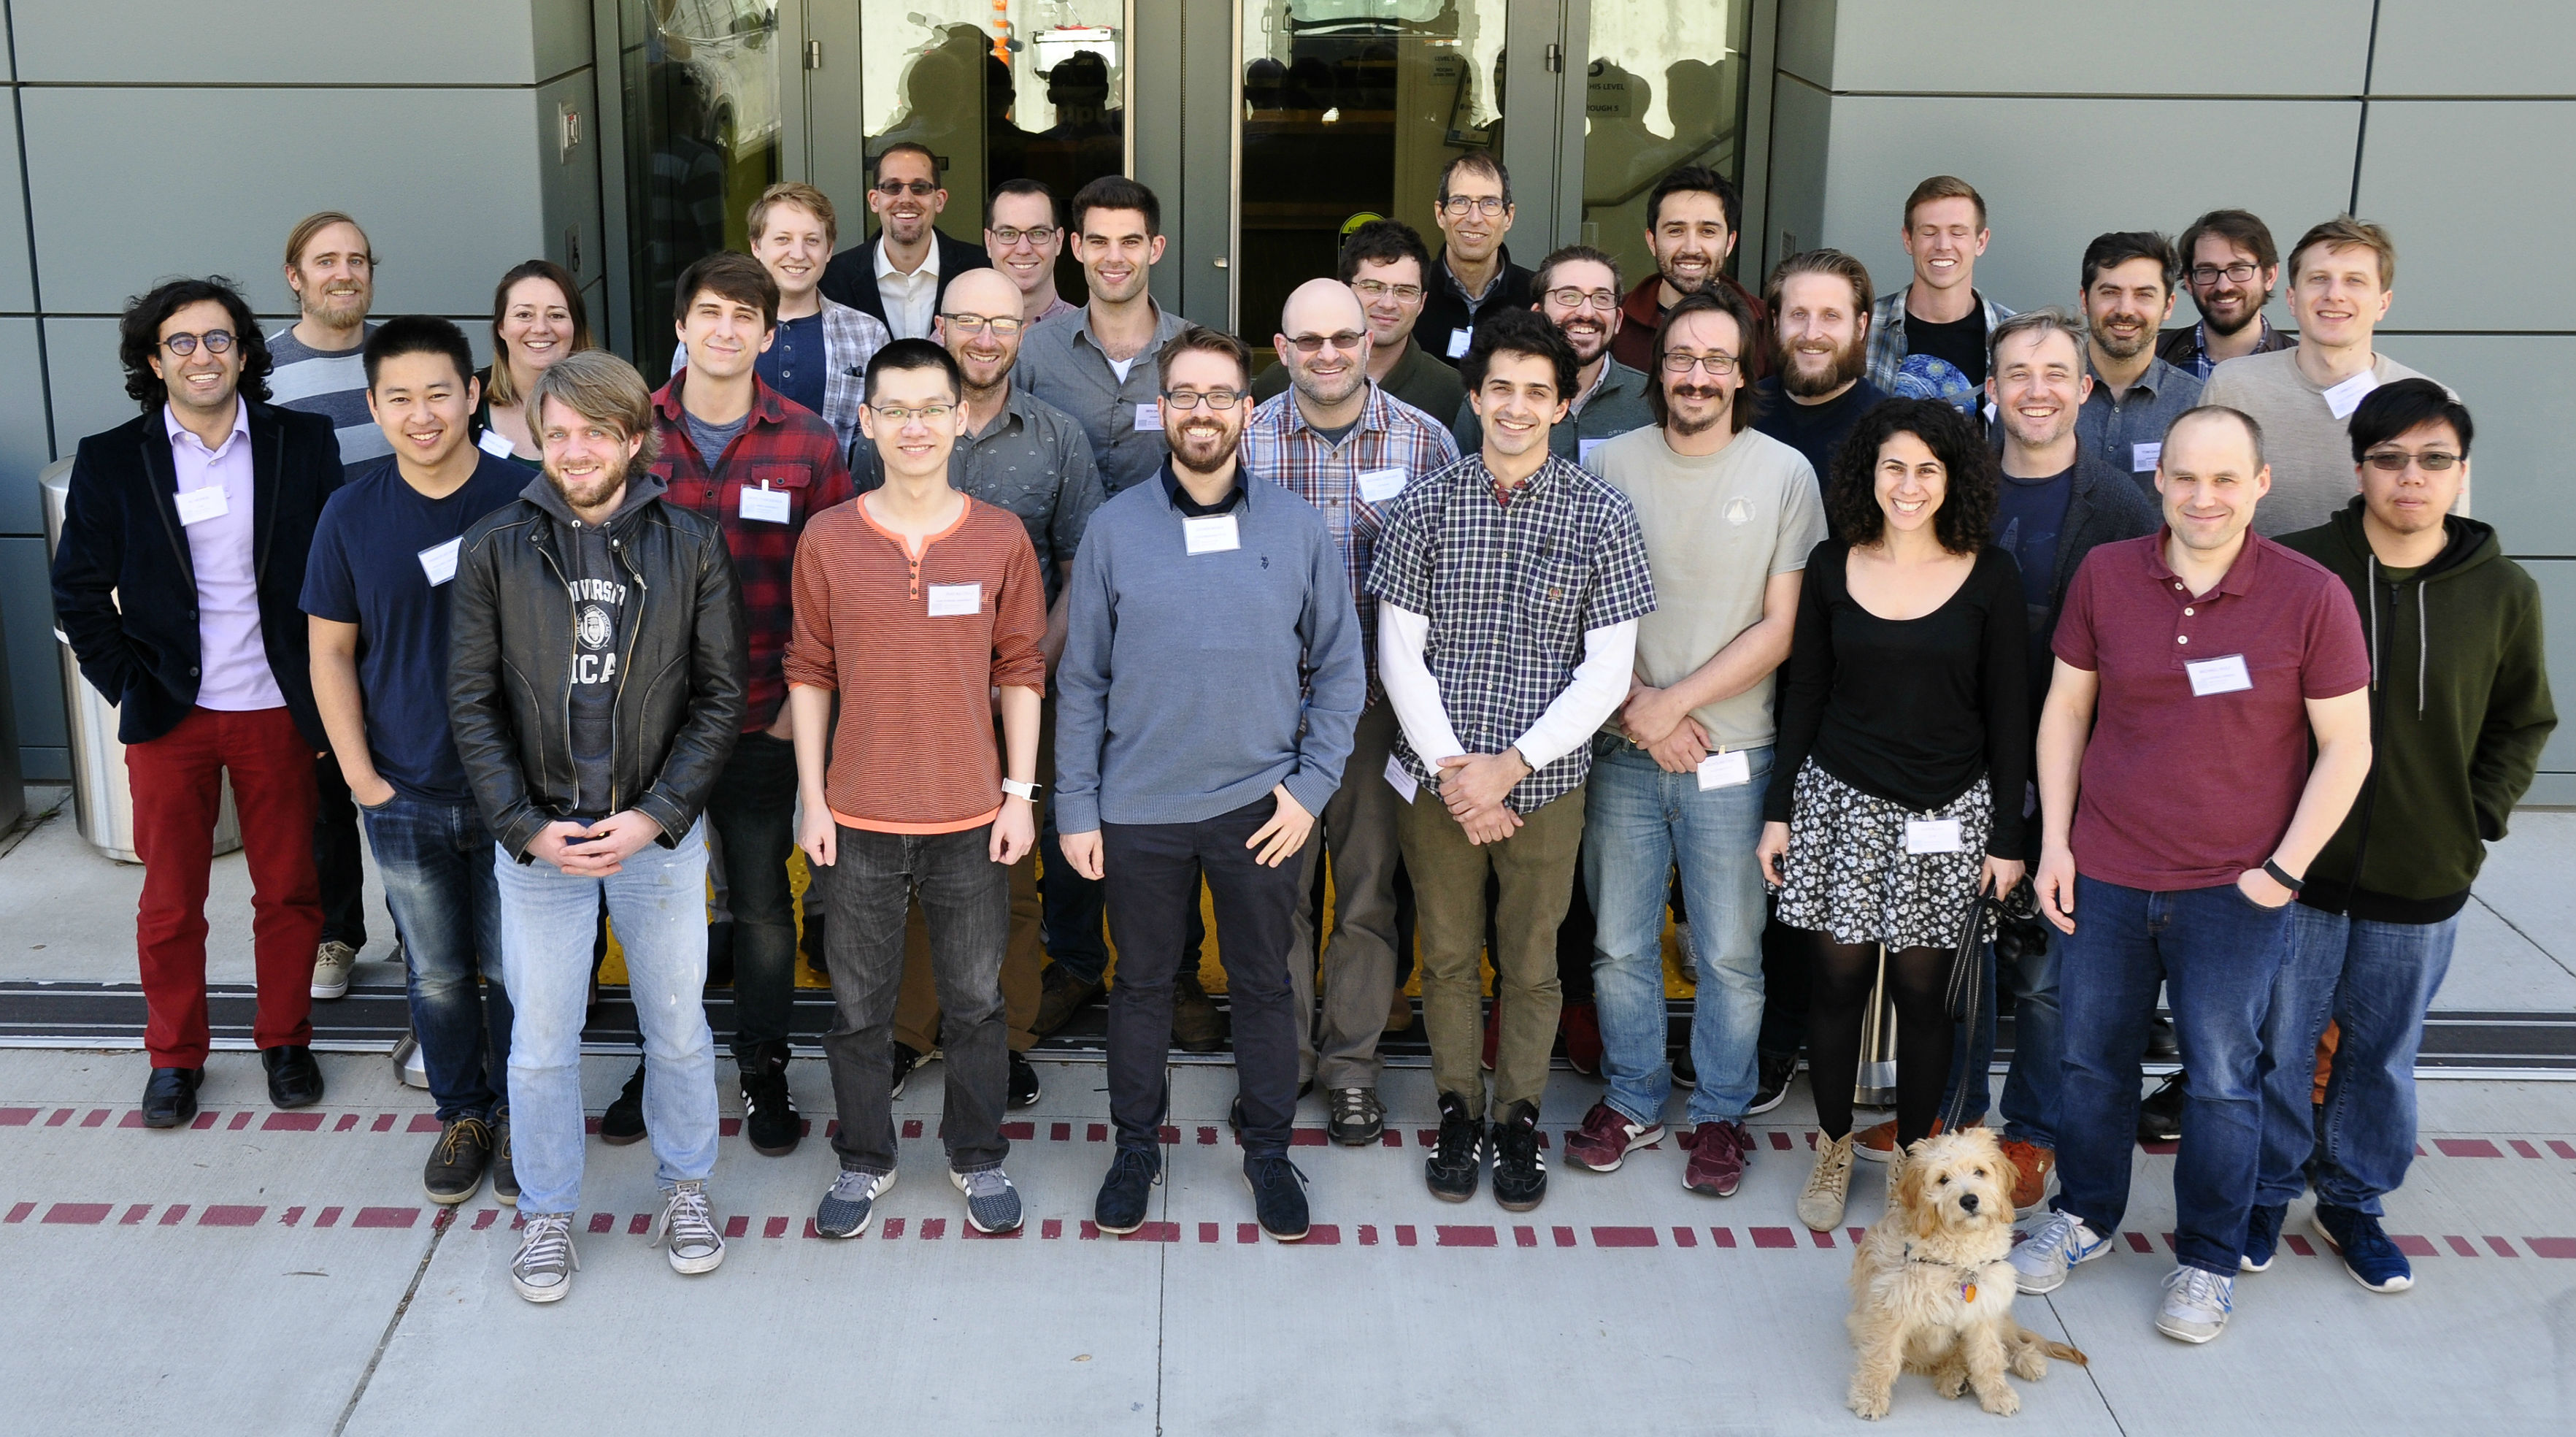
\includegraphics[width=\textwidth]{20180426-NWBN-Hackathon-Group-3.jpg}
\small \textit{Photo by Margie Wylie, Lawrence Berkeley National Laboratory} (see the \href{http://today.lbl.gov/2018/04/30/berkeley-lab-hosts-neurodata-without-borders-hackathon/}{LBNL News Release})
\end{staticcontents*}


%\begin{figure*}[h!]
%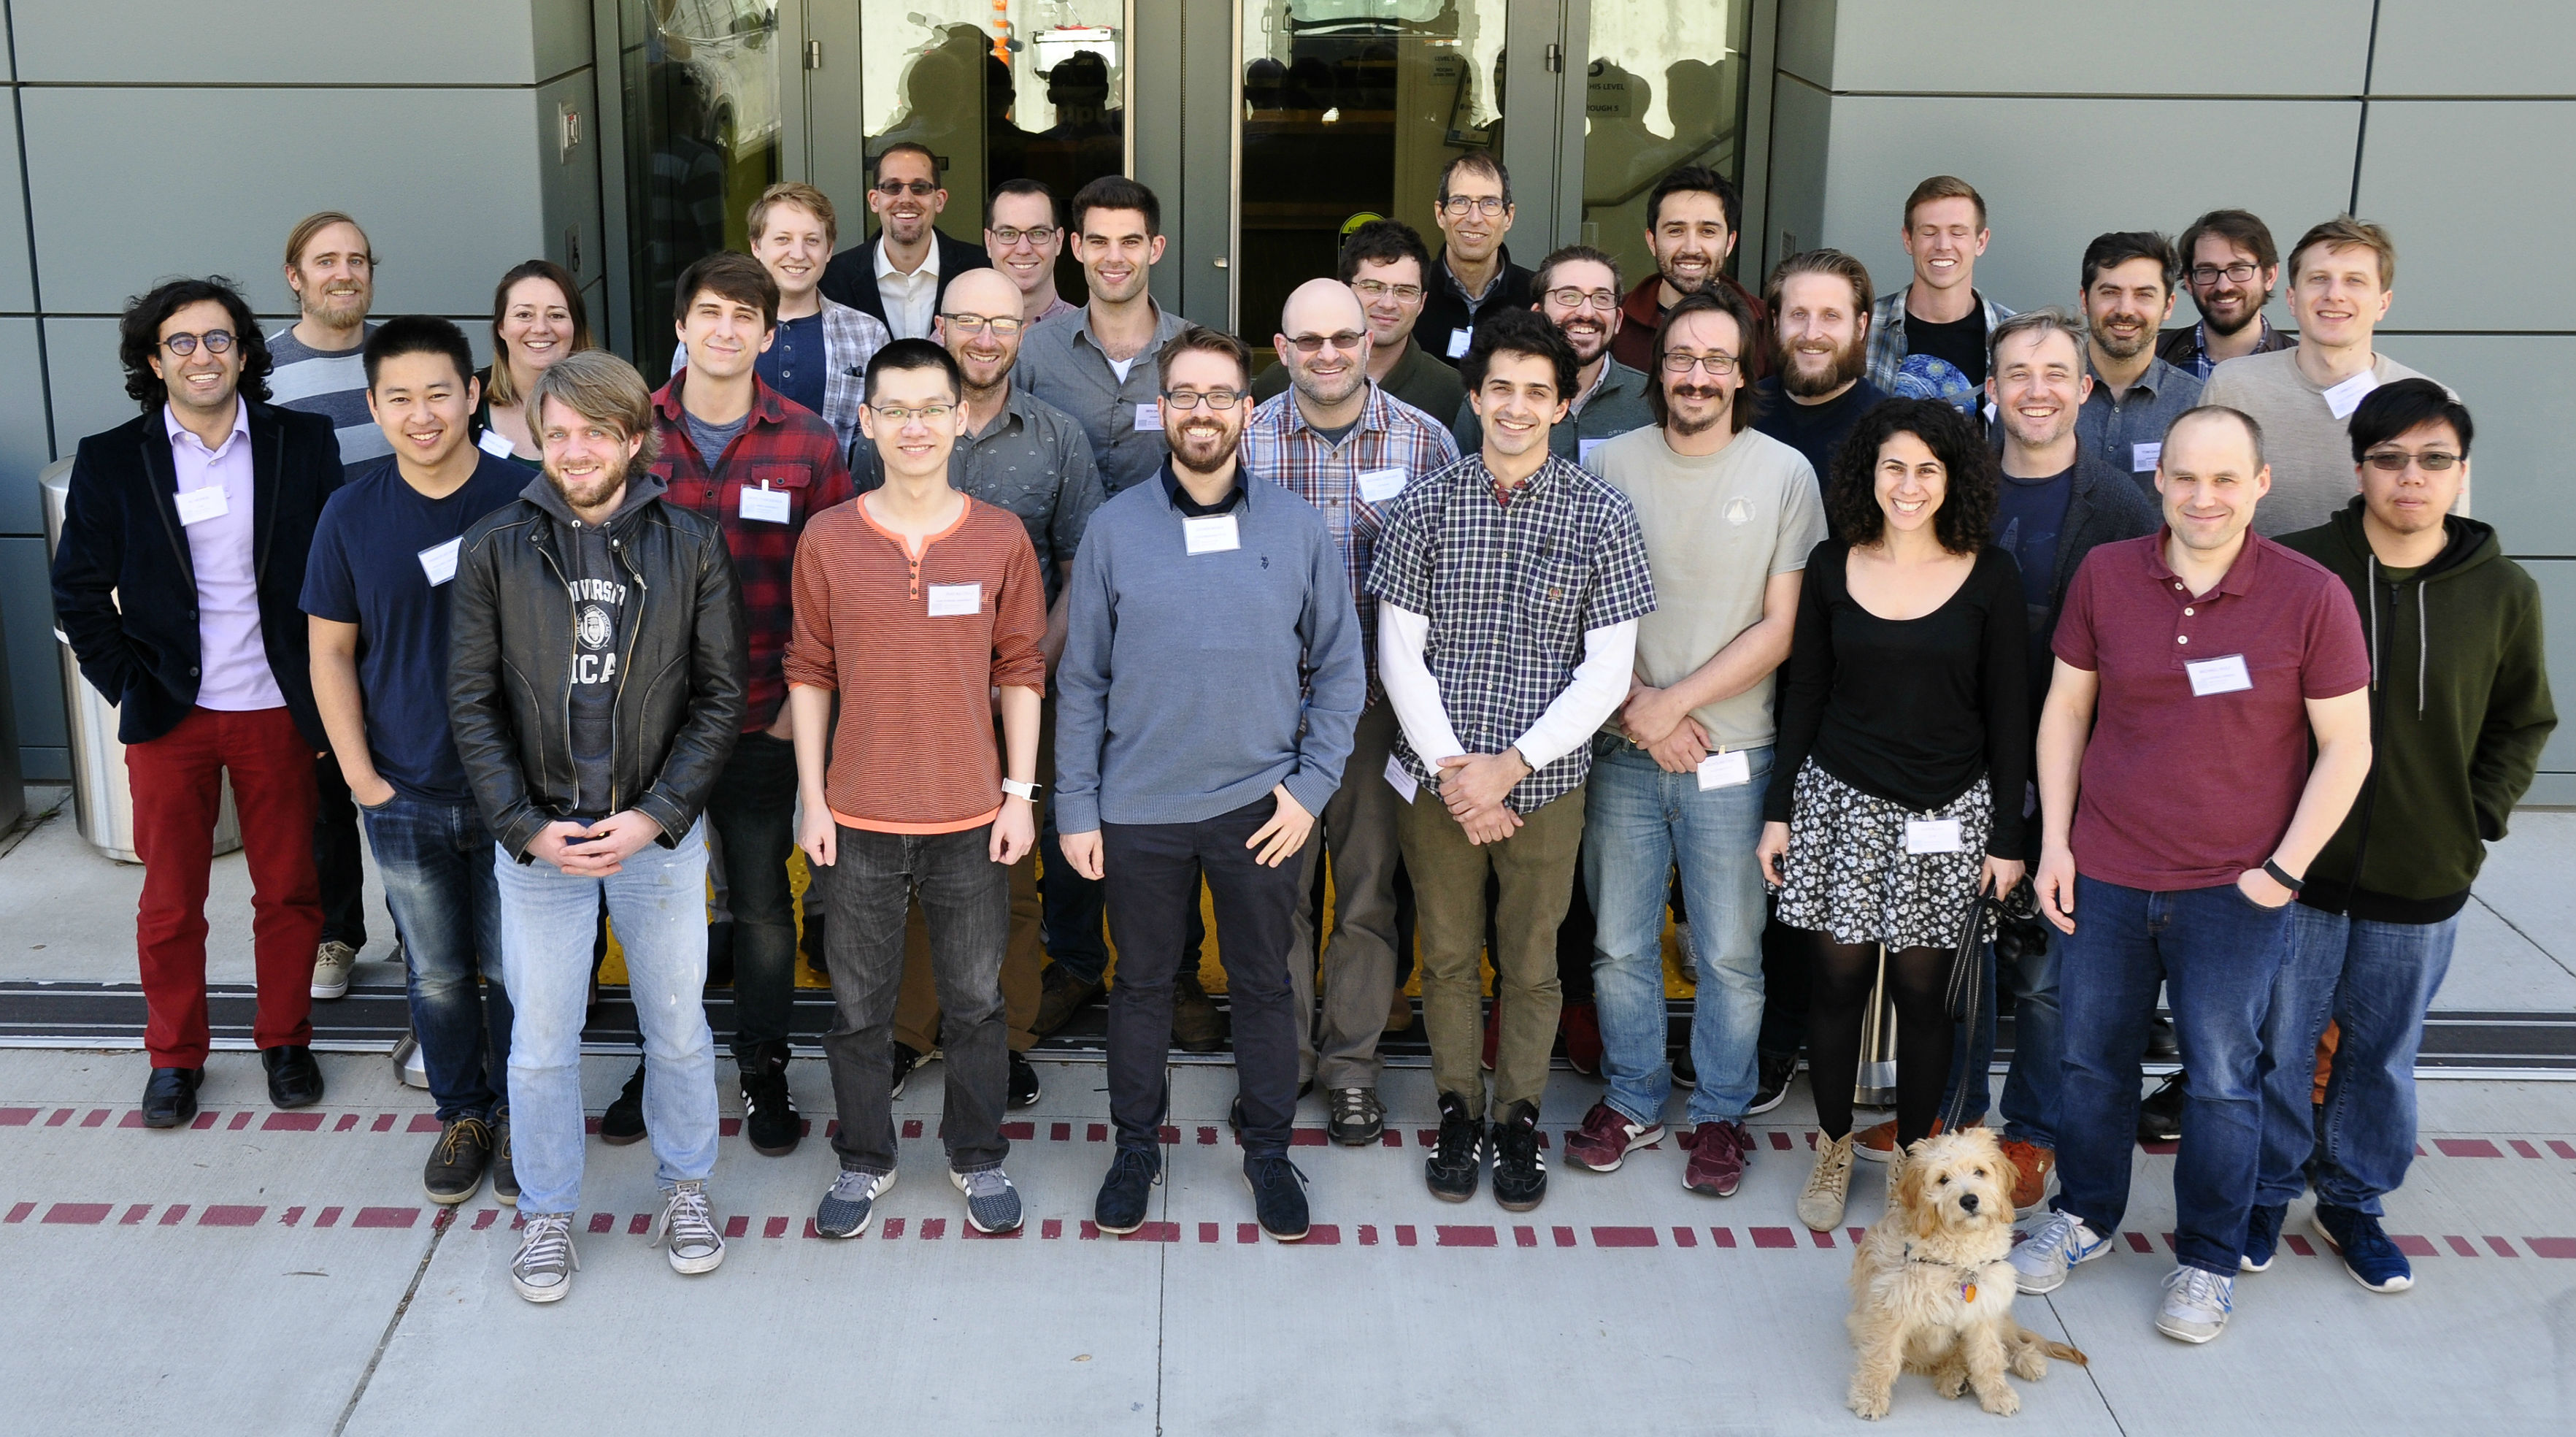
\includegraphics[width=\textwidth]{20180426-NWBN-Hackathon-Group-3.jpg}
%\end{figure*}


\tableofcontents
\clearpage

\section{Executive Summary}
\label{sec:es}

The \href{https://neurodatawithoutborders.github.io}{Neurodata Without Borders: Neurophysiology} 
(NWB:N) project is an effort to standardize the description and storage of 
neurophysiology data and metadata. NWB:N enables data sharing and reuse and 
reduces the energy-barrier to applying data analytics both within and across 
labs. %Several laboratories, including the Allen Institute for Brain Science, have wholeheartedly adopted NWB:N. The community needs to join forces to achieve data standardization in neurophysiology. 
This hackathon invited 
experts from the neuroscience community to explore adopting NWB:N for their
data sharing and analysis needs and lab use cases. The goal of this event was to: 
\textbf{a)} train new users on NWB:N, \textbf{b)} promote adoption of NWB:N, 
\textbf{c)} work with users on programming projects, e.g, to integrate examples
of their labs data into NWB:N, \textbf{d)} facilitate communication between users 
and developers and project teams, and \textbf{e)} engage with the community.

31 scientists from 13 major institutions and approximately 20 different labs/groups 
attended the event.  In addition, we had attendance by one friendly canine \smiley{}.
The background in programming varied greatly among the participants, ranging from beginners 
to experts. Most participants had investigated NWB:N prior to the event but
were generally in the early stages of exploration and adoption. 

During the coding sessions, participants worked on their \nameref{sec:userprojects},
which they had defined (and prepared) prior to the event. The user projects involved
data from a broad range of modalities:
\textbf{a)} electroyphysiology (voltage and current-clamp recordings,  ECoG),  
\textbf{b)} optophysiology,
\textbf{c)} static imaging modalities (2-photon imaging, fluorescent wide-field images, webcam, etc.,),
\textbf{d)} behavioral data,
\textbf{e)} processed data (e.g., from spike sorting),
\textbf{f)} neural simulations (Neuron),
\textbf{g)} stimulus data, and
\textbf{h)} trial-based data. The user projects also included data from a number of different 
species, such as, mice, rats, and monkeys.
See the \nameref{sec:userprojects} section for a more in-depth overview of the user projects
at the hackathon. 

In order to provide a balance between user training and project-oriented work, 
we designed the agenda to consist of an even split of talks (3h) and tutorials (4h20min) and hacking on user
projects (7h20min) (see the \nameref{sec:program}). Group discussions were held during lunch on 
    the first day for introduction and review of user hacking projects and at the end of the second 
day for review of progress, feedback, and discussion of the event. 

By the end of the hackathon, the vast majority of attendees had accomplished many of their goals,
and several were well on their way to having NWB:N fulfill their labs needs. All attendees 
indicated an enthusiasm for the current software and were impressed with the (relative) ease
of use given the generality. As an important step towards adoption, a few members 
(A. Milstein, S. Rolotti, J. Weber, M. Dougherty) indicated 
willingness to serve as 'tutors' for upcoming hackathon events: more effort is needed in the direction
of training members of the community to become trainers themselves. There was also consensus on 
a few features that would greatly enhance the utilization and adoptability of NWB:N:
\begin{itemize}
  \setlength\itemsep{0cm}
  \item \textbf{Extensions sharing:} The ability to share and use extensions across labs was recognized
  as a critical need. Formalizing and standardizing this process will be critical. This is already on
  the roadmap for NWB:N development as part of pending NIH proposals and was also part of the
  \href{https://neurodatawithoutborders.github.io/nwb_hackathons/HCK04_2018_Seattle/Projects/ExtensionSharing/}{Extension Sharing} project at the 4th hackathon at the Allen Institute . 
  \item \textbf{Controlled Vocabularies and Ontologies:} The ability to associate controlled terms 
   (e.g., enumerations) and complex ontologies with NWB:N data fields was recognized as a central need. 
   This is already on the roadmap for NWB:N development as part of pending NIH proposals. 
  \item \textbf{Tools for visualization and analysis:} Tools for exploration and
  visualization of NWB:N was recognized as a general need. Some development efforts are already 
  underway (e.g., Kitware, Gepetto etc.) but more efforts and integrated support for this are needed. 
  \item \textbf{Data search and query:} Advanced tools for search, discovery, and query of NWB:N
  data are needed to facilitate advanced data analytics. This is already on the roadmap for 
  NWB:N development as part of pending NIH proposals.
  \item \textbf{Trial-based data:} Support for trial-based data is currently limited in NWB:N
  and needs to be expanded (see \href{https://github.com/NeurodataWithoutBorders/nwb-schema/issues/152}{Issue \#152})
\end{itemize}
These should be targets for future development efforts. See also the \nameref{sec:es:dev} section
for additional (lower-level) specific developments suggested by attendees at the hackathon.

Overall, the hackathon was a great success. Based on discussions at the hackathon the suggestion is to 
ideally have similar, user-oriented hacking events approximately every 6 month, 
at least at this early stage of development/adoption of NWB:N 2. 

\vspace{2cm} 
\subsection{Suggestions for Future Events}
\begin{itemize}
  \setlength\itemsep{0cm}
  \item \textbf{The hackathon was very useful:} Nearly all participants    
     indicated that they would be willing to attend another NWB:N 
     hacking event in the future. All participants appeared to have
     made significant progress on their projects during the event. 
  \item \textbf{Desire for even more time for project hacking:}
     Tom Davidson and other attendees indicated that a central 
     value of the event is to get people in the same room. In general 
     participants indicated a desire for more time for programming 
     and working on projects.
  \item \textbf{2 days is a good length for the event:} 
      The overall length of the meeting of 2 days appeared to have 
      been perceived as good, in part because it provides a compromise
      between the busy schedules of participants and the value-add from
      a hacking event. In that regard, Nathan Clack and others suggested
      to have shorter/less talks to accommodate more project sessions.
       In addition, another option may be to have an 
       optional third day
      just for project hacking and working groups.
   \item \textbf{Consider adding breakout sessions:} 
      With regard to the issue of allowing for more hacking, 
      it was suggested to have breakout sessions on particular topics 
      (e.g., ephys, ophys, advanced I/O etc.) to enable attendees to 
      focus on the topics that are of most value to them while at the
      same time allowing us to cover a broad range of topics.
   \item \textbf{Consider alternate name for the event:} Karen Lavi
      (UCSF) suggested that the term "Hackathon" may pose a hurdle for
      diversity. To attract more female attendees she suggested that
      the event should be renamed to be more open and welcoming. 
      In the series of hackathons, this was really the first
      event that focused on user training and community engagement.
      As such, we may want use the term hackathon for
      developer events and create a new name for training and
      engagement events that better reflects the user/community
      focus. In general encouraging more diversity and participation
      of women and minorities will be useful. 
   \item \textbf{Consider adding code/file review groups:}
      Jochen  Weber (ZMBBI) suggested to add code/file review sessions
      in which participants would be paired with one (or more) 
      participants from other lab, to review codes (generated at the 
      event) in pairs or small subgroups to provide feedback, 
      facilitate communication, and help prepare  data (and codes) for
      sharing and typical use cases in other labs.
   \item \textbf{Satellite events:} The option of holding satellite tutorial, training,
      and community engagement events at major neuroscience conferences was also mentioned, 
      specifically SfN and Cosyne. 
\end{itemize}

\subsection{Suggestions for Specific Developments}
\label{sec:es:dev}

In addition to the more high-level direction for future development discussed in the 
\nameref{sec:es} we here describe additional, specific developments that were suggested
by participants at the hackathon. 

\begin{itemize}
 \setlength\itemsep{0cm}
 \item \textbf{Create simple end-to-end tutorial:} Create a tutorial that shows the creation of an 
      extension and its use for write and read on real data. {\footnotesize \href{https://github.com/NeurodataWithoutBorders/pynwb/issues/505}{https://github.com/NeurodataWithoutBorders/pynwb/issues/505}}
 \item \textbf{Improve support for trial data}: {\footnotesize  \href{https://github.com/NeurodataWithoutBorders/nwb-schema/issues/152}{https://github.com/NeurodataWithoutBorders/nwb-schema/issues/152}}
 \item \textbf{Ways to browse through NWB:N files:} Improve introspection, search, query, and visualization capabilities.
 \item \textbf{Event data:} Specialize for ripple, downstate
 \item \textbf{Interfacing visualization and analysis tools with NWB:N:} E.g., Neuroscope (C/C++). Read NWB data
      for kilosort, mclust, neurosuite.
 \item \textbf{Cache the Specification:} Cache the specification (including extensions) always to the file. This
      suggestion also related to the desire for formal mechanisms for sharing extensions. 
 \item \textbf{Communicate mission of NWB:N:} Should NWB:N be used only for sharing of data 
        or day-to-day use? Answer: goal is day-to-day.
 \item \textbf{Multi-plane imaging:} Storing multi-plane imaging data is not optimally supported in NWB:N yet. In
        particular, ROIs sometimes span imagine planes in this context. 
 \item \textbf{Neuron data:} Made a lot of progress already. 
 \item \textbf{Enable modeling of data constraints for validation:} This could be either part of the schema
       language or part of a separate validation model to define additional data constraints. Currently this
       functionality is implemented by the API classes but should be formalized to ensure consistency of
       constraints cross languages/APIs.
 \item \textbf{Facilitate integration/linking to data in non-NWB:N files:} To ease adoption at labs some
       labs would like to link to custom external file formats (e.g., binary data) to avoid data copy and
       allow use of existing lab software tool-chains on existing data. In PyNWB this could be accomplished
       via custom I/O backends as well as via customization of the ObjectMapper API.
 \item \textbf{Iterative Write (PyNWB):} Works
 \item \textbf{Lazy load (PyNWB):} Works 
\end{itemize}

\noindent Several Matlab-specific suggestions included:
\begin{itemize}
  \item \textbf{Continue to support Matlab:} Attendees at the event estimated that $\approx 50\%$ of target 
        users are currently MATLAB users.
  \item \textbf{MatNWB: Consistent ordering of dimensions:} Dimensions in Matlab are ordered
        differently from Python. Make this consistent to follow the spec. 
        {\scriptsize \href{https://github.com/NeurodataWithoutBorders/matnwb/issues/26}{https://github.com/NeurodataWithoutBorders/matnwb/issues/26} }
 \item \textbf{MatNWB: Support lazy data load:} {\footnotesize \href{https://github.com/NeurodataWithoutBorders/matnwb/issues/27}{https://github.com/NeurodataWithoutBorders/matnwb/issues/27}}

\end{itemize}

\subsection{Survey}

All participants were asked to participate in an exit survey. 8 participants (i.e., $~26\%$) submitted responses
to the survey. The following figure summarizes the results of the survey questions in which users were asked to
rate the hackathon and software using a numeric scale ranging from 1 (worst) to 5 (best). 

\begin{figure*}[h!]
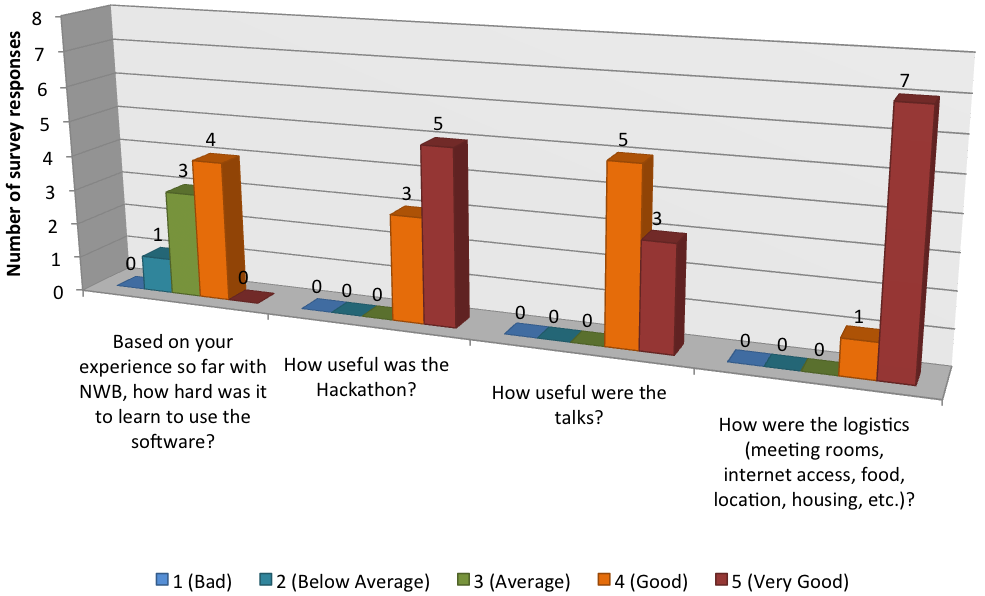
\includegraphics[width=15.5cm]{survey_chart.png}
\label{fig:survey}
\end{figure*}

\clearpage
\section{Organization}

The meeting was organized by Oliver Ruebel (site/program chair), Andrew Tritt and Kristofer Bouchard with administrative support by Dionne Myers and additional logistics support by Stephanie Albin (Kavli Foundation). Travel support for the meeting was provided by the KAVLI Foundation and food and other meeting resources were sponsored by Lawrence Berkeley National Laboratory. 


\begin{figure*}[h!]
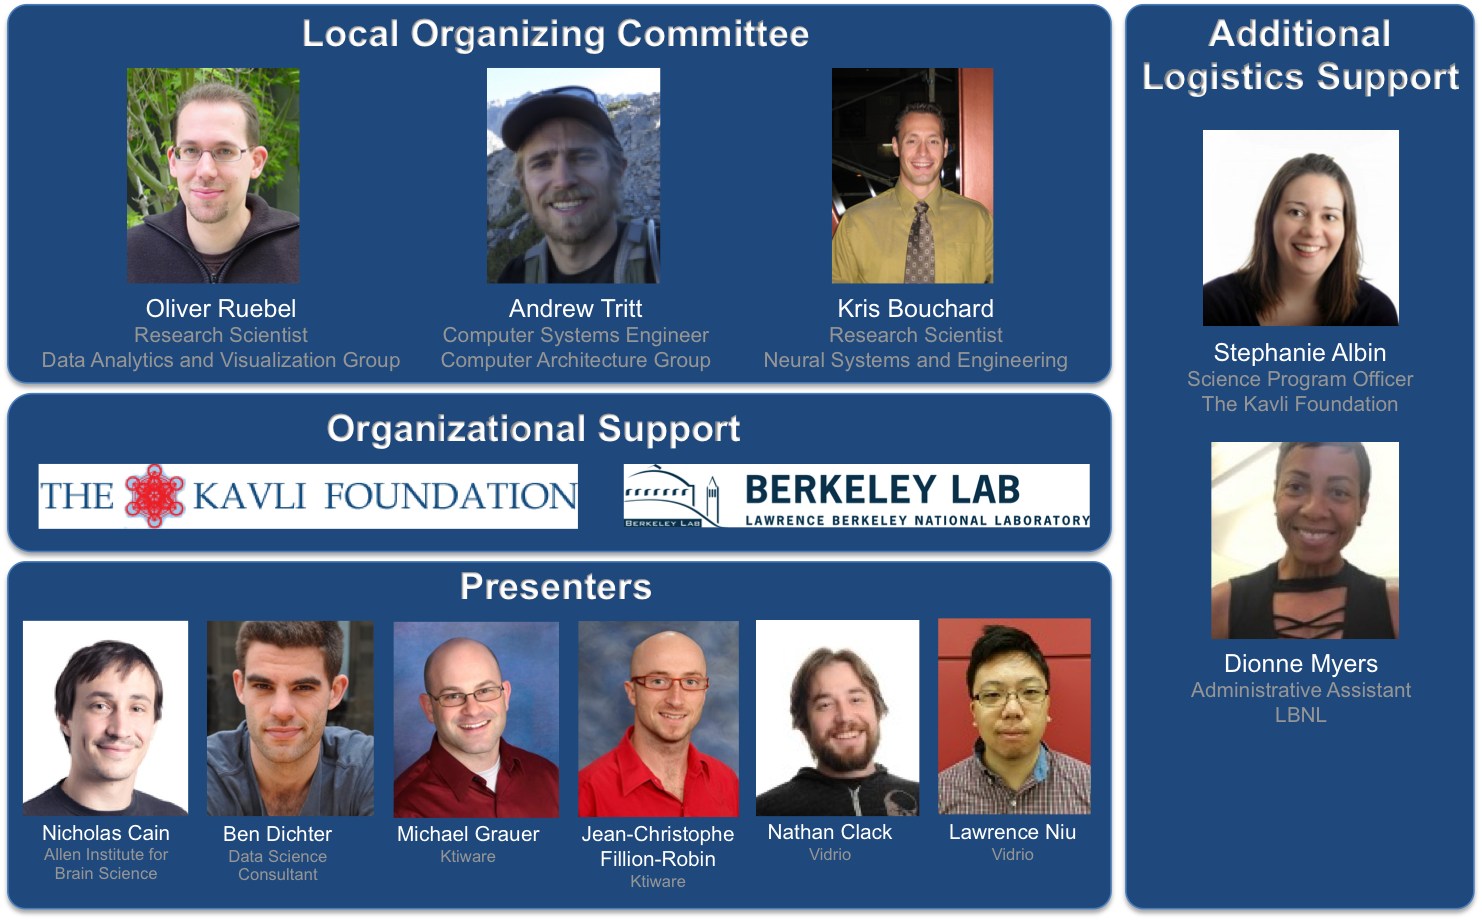
\includegraphics[width=15.5cm]{nwb_hackathon_presenters.png}
\end{figure*}

\clearpage

\section{Program}
\label{sec:program}

\begin{itemize}
  \item \textbf{Event Website:} \href{https://neurodatawithoutborders.github.io/nwb_hackathons/HCK05_2018_Berkeley}{https://neurodatawithoutborders.github.io/nwb\_hackathons/HCK05\_2018\_Berkeley}
  \item \textbf{Dates:} April 26-27, 2018
  \item \textbf{Location:} Lawrence Berkeley National Laboratory, Berkeley, CA, USA, Building 59 - Shyh Wang Hall %, Room 4102 (main meeting room), 4101 (Food and Breakouts), 4016 (Day 1 breakouts), 3049 (Day 2 breakouts)
  \item \textbf{Slides:} The slides from the talks and tutorials presented at the event are available online at: \\ \href{https://neurodatawithoutborders.github.io/nwb_hackathons/HCK05_2018_Berkeley/#slides}{https://neurodatawithoutborders.github.io/nwb\_hackathons/HCK05\_2018\_Berkeley/\#slides}
\end{itemize}


\subsection{Breakdown of Event Times}
\label{sec:program:breakdown}

\begin{table}[h!]
\small
%\centering
\label{tab:event:times}
\begin{tabular}{|l|l|l|l||l|}
\hline
                                          &                     & \textbf{Day 1}    & \textbf{Day 2}   & \textbf{Totals across both days} \\\hline
\textbf{Talks}                            & \cellcolor{blue!}   & 2:30:00           & 0:30:00          & \textbf{3:00:00}                 \\\hline
\textbf{Tutorials with hacking exercises} & \cellcolor{yellow!} & 1:30:00           & 2:50:00          & \textbf{4:20:00}                          \\\hline
\textbf{Hacking on user projects}         & \cellcolor{lime!} & 4:10:00           & 3:10:00          & \textbf{7:20:00}                          \\\hline
\textbf{Breaks}                           & \cellcolor{gray!25} & 1:50:00           & 2:00:00          & \textbf{3:50:00}                         \\\hline
\textbf{Group Discussion}                 & \cellcolor{gray!25} & 0:10:00           & 1:00:00          & \textbf{1:10:00}                          \\\hline \hline
\textbf{Totals per day}                   &                     & \textbf{10:10:00} & \textbf{9:30:00} &                                  \\\hline
\end{tabular}
\end{table}
\vspace{-0.3cm}

\subsection{Agenda: Day 1}
\vspace{-0.1cm}
\textbf{Day 1: Thursday April, 26}
\vspace{-0.2cm}
\begin{table}[h!]
\small
\centering
\label{tab:program:day1}
\begin{tabular}{|l|l|p{6cm}|p{2cm}|p{1.5cm}|l|}
\hline
\textbf{Time}       & \textbf{Duration} & \textbf{Topic}                                                                               & \textbf{Speaker}         & \textbf{Room}                               & \textbf{}           \\ \hline \hline
7:30 - 8:00       & 0:30:00           & Registration \& Breakfast                                                                      &                          & 59-4101                                     & \cellcolor{gray!25}  \\ \hline
8:00 - 8:10       & 0:10:00           & Welcome to the NWB:N Hackathon @ LBNL                                                          & Oliver Ruebel            & 59-4102                                     & \cellcolor{blue!} \\ \hline
8:10 - 8:20       & 0:10:00           & Neurodata Without Borders - Standardization of neurophysiology data ...                        & Kris Bouchard            & 59-4102                                     & \cellcolor{blue!} \\ \hline
8:20 - 8:40       & 0:20:00           & Introduction to NWB:N – An ecosystem for standardizing neurophysiology data                    & Oliver Ruebel            & 59-4102                                     & \cellcolor{blue!} \\ \hline
8:40 - 9:40       & 0:30:00           & NWB:N and PyNWB – A Python API for standardizing neurophysiology data                          & Andrew Tritt             & 59-4102                                     & \cellcolor{blue!} \\ \hline
9:40 - 10:10      & 0:30:00           & Overview of MatNWB                                                                             & Nathan Clack, Lawrence Niu   & 59-4102                                 & \cellcolor{blue!} \\ \hline
10:10 - 10:25     & 0:15:00           & Break                                                                                          &                          & 59-4101, 59-4102                            & \cellcolor{gray!25} \\ \hline
10:25 - 11:10     & 1:30:00           & NWB:N I/O – ophys                                                                              & Nicholas Cain               & 59-4102                                     & \cellcolor{yellow!}   \\ \hline
10:10 - 11:55     & 1:30:00           & NWB:N I/O – ephys                                                                              & Ben Dichter              & 59-4102                                     & \cellcolor{yellow!}   \\ \hline
11:55  - 12:30    & 0:30:00           & Tour of the National Energy Research Scientific Computing Center (Optional)            &                          & 59-4102, NERSC                              & \cellcolor{gray!25}\\ \hline
11:55 - 1:00      & 1:05:00           & Working Lunch with presentation on: Expectations and Overview of Hackathon Projects            & Oliver Ruebel            & 59-4101, 59-4102                            & \cellcolor{gray!25} \\ \hline
1:00 - 3:00       & 2:00:00           & Hacking on projects                                                                            &                          & 59-4101, 59-4102, 59-4016                   & \cellcolor{lime} \\ \hline                    
3:00 - 3:10    & 0:10:00              & Group Photo                                                                                    &                          & Entrance 59                                 & \cellcolor{gray!25}  \\ \hline
3:10 - 3:30       & 0:20:00           & Break                                                                                          &                          & 59-4101, 59-4102                            & \cellcolor{gray!25}  \\ \hline
3:30 - 5:40       & 2:10:00           & Hacking on projects                                                                            &                          & 59-4101, 59-4102, 59-4016                   & \cellcolor{lime} \\ \hline  
6:30              & 2:00:00           & Group Dinner (Optional)                                                                        &                          & Triple Rock (1920 Shattuck Avenue) & \cellcolor{gray!25}  \\ \hline
\end{tabular}
\end{table}


\subsection{Agenda: Day 2}
\vspace{-0.1cm}
\textbf{Day 2: Friday April, 27}
\vspace{-0.2cm}
\begin{table}[h!]
\small
\centering
\label{tab:program:day2}
\begin{tabular}{|l|l|p{6cm}|p{2cm}|p{1.5cm}|l|}
\hline
\textbf{Time}       & \textbf{Duration} & \textbf{Topic}                                                                               & \textbf{Speaker}         & \textbf{Room}                               & \textbf{}           \\ \hline \hline
8:30 - 9:30         & 0:30:00           & Breakfast                                                                                    &                          & 59-4101                                     & \cellcolor{gray!25}  \\ \hline
9:00 - 9:10         & 0:10:00           & Welcome to Day 2 of the NWB:N Hackathon @ LBNL                                               &  Oliver Ruebel           & 59-4102                                     & \cellcolor{blue!}  \\ \hline
9:10 - 9:30         & 0:20:00           & PyNWB Software Process and How to Contribute                                                 &  Michael Grauer, Jean-Christophe Fillion-Robin     & 59-4102           & \cellcolor{blue!}  \\ \hline
9:30 - 10:30        & 1:00:00           & Writing Extensions                                                                           &  Ben Dichter             & 59-4102                                     & \cellcolor{yellow!}  \\ \hline
10:30 - 10:45       & 0:15:00           & Break                                                                                        &                          & 59-4101, 59-4102                            & \cellcolor{gray!25} \\ \hline
10:45 - 11:45       & 1:00:00           & PyNWB Containers – Front-end objects for NWB data                                            &  Andrew Tritt            & 59-4102                                     & \cellcolor{yellow!}  \\ \hline
11:55 - 1:00        & 1:15:00           & Working Lunch with presentation on: Advanced Data I/O                                        &  Oliver Ruebel           & 59-4101, 59-4102                            & \cellcolor{gray!25} \\ \hline
1:00 - 1:30         & 0:30:00           & Advanced Data I/O (Hacking exercises)                                                        &  Oliver Ruebel           & 59-4102                                     & \cellcolor{yellow} \\ \hline                    
1:30 - 3:00         & 1:30:00           & Hacking on projects                                                                          &                          & 59-4101, 59-4102, 59-3049                   & \cellcolor{lime} \\ \hline                    
3:00 - 3:20         & 0:20:00           & Break                                                                                        &                          & 59-4101, 59-4102                            & \cellcolor{gray!25}  \\ \hline
3:20 - 5:00         & 1:40:00           & Hacking on projects                                                                          &                          & 59-4101, 59-4102, 59-3049                   & \cellcolor{lime} \\ \hline  
5:00 - 6:00         & 1:00:00           & Group Discussion (Review of progress and feedback)                                            &                         & 59-4101 & \cellcolor{gray!25}  \\ \hline

\end{tabular}
\end{table}


\clearpage
\section{User Projects}
\label{sec:userprojects}

Prior to the event, each participant was asked by the organizers to formulate a specific project that 
she/he will work on. The participants created project pages on the \href{https://github.com/NeurodataWithoutBorders/nwb_hackathons/tree/master/HCK05_2018_Berkeley/projects}{hackathon GitHub repository}. Participants then updated
their pages during (and after) the event to document progress. The tables on the following pages provide
an overview of the various user projects. The project headings include links to the specific project pages
for further details. 


\vspace{1cm}
\begin{tabular}{|p{8cm}|p{2cm}|p{3.5cm}|}
\hline
\thead{\textbf{Title}}   & \thead{\textbf{Key} \\ \textbf{Investigators}}   &  \thead{\textbf{Key} \\ \textbf{Institutions}} \\ \hline \hline
\textbf{\href{https://neurodatawithoutborders.github.io/nwb_hackathons/HCK05_2018_Berkeley/projects/ZMBBI/}{NWB Camera Capture code}} This project will investigate the use of the NWB framework to compile data from multiple sources and formats into a single NWB file. This data includes intrinsic and fluorescent wide-field images from awake behaving mice, as well as behavioral webcam images to accompany it. We hope to construct an NWB file, import the data into the file, and then read it into a matlab workspace for later analysis. & \makecell{Jochen Weber, \\ David Nicholas} & Zuckerman Mind Brain Behavior Institute, Columbia University \\ \hline
\textbf{\href{https://neurodatawithoutborders.github.io/nwb_hackathons/HCK05_2018_Berkeley/projects/GrangerProject/}{Conversion of Sabatini lab neurophysiology and imaging data to the NWB:N format}} The goal of this project is to convert the whole-cell electrophysiology data from the Sabatini lab to the NWB format. This data includes voltage-clamp and current-clamp recordings from neurons in acute brain slices. This data is typically analyzed for the presence or absence of synaptic responses or changes in membrane potential. However, we often extract other features such as response amplitude, latency, onset and offset kinetics, frequency of synaptic events or action potentials, and variability of responses in repeated trials. Therefore, a standard toolset to analyze this data in the NWB data format would also be useful. Finally, we often record electrophysiology data in tandem with 2-photon imaging, and would like to be able to incorporate imaging data into the NWB:N file format.   & \makecell{Adam Granger}   &  Sabatini Lab, Harvard Medical School \\ \hline
\textbf{\href{https://neurodatawithoutborders.github.io/nwb_hackathons/HCK05_2018_Berkeley/projects/LosonczyLab/}{Conversion of multimodal data between Losonczy Lab and NWB:N formats}} Our lab collects 2-photon imaging and extracellular electrophysiological data in awake behaving mice. Our overall goal is to increase the interoperability of our data structures and formats with those of NWB. We already have fairly well developed repositories for working with our data, including a public package for sequential imaging data (SIMA) as well as in-house lab analysis bundle (LAB) for associating and analyzing these various data formats. We therefore hope to allow for seamless import from and export to NWB using the APIs for these repos.  & \makecell{Sebi Rolotti}  &  Losonczy Lab, Columbia University \\ \hline
\textbf{\href{https://neurodatawithoutborders.github.io/nwb_hackathons/HCK05_2018_Berkeley/projects/Buzsakilab/}{Integrating Buzcode standard into NWB}} & David Tingley  &  Buzsaki Lab, New York University  \\ \hline
\end{tabular}

\begin{tabular}{|p{8cm}|p{2cm}|p{3.5cm}|}
\hline
\thead{\textbf{Title}}   & \thead{\textbf{Key} \\ \textbf{Investigators}}   &  \thead{\textbf{Key} \\ \textbf{Institutions}} \\ \hline \hline
\textbf{\href{https://neurodatawithoutborders.github.io/nwb_hackathons/HCK05_2018_Berkeley/projects/DAtagging/}{A database of dopamine cell recordings in freely-moving rats}} Recordings of dopamine cells in behaving animals have been enormously influential in neuroscience, psychology, and even computer science. In head-restrained monkeys and mice performing passive tasks, dopamine cells appear to encode reward prediction errors (RPEs) - abrupt changes in the anticipation of future rewards. RPE signals are central to reinforcement learning algorithms, and are a core component of recent advances in artificial intelligence (e.g. AlphaGo). However, there is more and more data indicating that RPEs are an incomplete description of dopamine function, including recent results from our laboratory (Hamid et al. 2016, Nature Neuroscience). As part of our ongoing dopamine studies we have been recording from optogenetically-identified dopamine cells ($n > 33$) in the rat ventral tegmental area. These are - to our knowledge - the first recordings of identified dopamine cells in unrestrained animals performing distinct behavioral tasks, including a probabilistic reward (“bandit”) task, a runway task, and a pavlovian approach task. Initial analyses suggest that the RPE idea is a good description of some aspects of dopamine cells firing, but not others. This unique, high-quality data set is certain to be of great interest to many researchers, especially computational neuroscientists who do not perform their own recordings. We wish to convert this dopamine data, with associated behavioral and anatomical metadata, into the NWB format as an important step towards freely-distributing these data to the community.  & 
    \makecell{ Ali Mohebi, \\ Josh Berke}   &  University of California San Francisco (UCSF)  \\ \hline  
\textbf{\href{https://neurodatawithoutborders.github.io/nwb_hackathons/HCK05_2018_Berkeley/projects/FilterReadByLabel/}{Filter Read by Label}} We would like to define a standard way to associate data points in an NWB file with multiple user-defined categorical labels, and then be able to selectively read from a dataset just the data points that satisfy a boolean filter based on those labels. An example would be a dataset of UnitTimes containing spike trains recorded from an extracellular electrophysiology experiment. Each neuron in the dataset could be assigned a categorical label according to its 1) cell\_type, 2) feature\_selectivity (grid cell or head direction cell?), 3) active during sleep / wake?, etc. Then the user could read into memory the spikes from all cells that match a query for ‘cell\_type’ == ‘basket\_cell’, ‘selectivity’ == ‘running\_speed’, ‘behavioral\_state’ == ‘sleep’, e.g. & \makecell{Aaron Milstein, \\ Ivan Raikov, \\ Ben Dichter} &  Standford University  \\ \hline
\textbf{\href{https://neurodatawithoutborders.github.io/nwb_hackathons/HCK05_2018_Berkeley/projects/OConnorLabCrossmodal}{O’Connor Lab’s Crossmodal Attention Project}} Conversion of extracellular electrophysiology data from our crossmodal attention project to the NWB:N format &  \makecell{Eric Finkel}   &  Johns Hopkins School of Medicine, O’Connor Lab \\ \hline
 \textbf{\href{https://neurodatawithoutborders.github.io/nwb_hackathons/HCK05_2018_Berkeley/projects/SohalLab/}{Calcium imaging of PFC neurons during Open Field paradigm}} The goal of this project is to assess the conversion of neuronal data of the Sohal lab to the NWB format. The data of this POC project includes in-vivo calcium imaging from PFC neurons in freely behaving mice in the open field aperture. A time series of the animal’s position within the aperture is also included. Currently, our lab is using in house solutions for working with data in Matlab. Here we hope to allow seamless import and export to NWB using the available APIs. & Karen Lavi, Scott Wilke &  Sohal lab, University of California San Francisco (UCSF)  \\ \hline
\end{tabular}

\begin{tabular}{|p{8cm}|p{2cm}|p{3.5cm}|}
\hline
\thead{\textbf{Title}}   & \thead{\textbf{Key} \\ \textbf{Investigators}}   &  \thead{\textbf{Key} \\ \textbf{Institutions}} \\ \hline \hline
\textbf{\href{https://neurodatawithoutborders.github.io/nwb_hackathons/HCK05_2018_Berkeley/projects/PesaranLabMultiModal/}{Conversion of Pesaran lab electrophysiology data to the NWB:N format}} The goal of this project is to convert local field potential and spike time data from the Pesaran Lab to the NWB format. This data includes behavioral data from awake, behaving Rhesus Macaques. This data is typically analyzed by aligning spike times or local field potential data to behavioral events of interest, such as the initiation of a saccade. Therefore, it would be useful to have a clean mechanism for associating data from combinations of arbitrary behavioral conditions (e.g. a saccade to the left during an instructed delay task two-alternative forced choice task), user-defined data conditions (e.g. spike time data from cells tuned to saccade direction from electrodes in the lateral intraparietal sulcus) at user-specified events (e.g. the beginnning of an optogenetic stimulation sequence). As our lab continues to extend recording modalities (e.g. to 2-photon calcium imaging), it would also be useful to have the ability to seamlessly integrate new data formats and types.
Our lab has previously developed in house solutions for working with the above data in Matlab. Here we hope to allow seamless import and export to NWB using the available APIs. & \makecell{Kevin Brown, \\ Bijan Pesaran}                           &   Pesaran lab, New York University  \\ \hline
\textbf{\href{https://neurodatawithoutborders.github.io/nwb_hackathons/HCK05_2018_Berkeley/projects/KepecsLab/}{Converting e-phys/behavioral data into NWB:N data format (Kepecs lab)}} This project aims to convert electrophysiological, imaging and behavioral data into the nwb data format. Data was obtained from different projects in Adam Kepecs’ lab at CSHL. We made progress converting voltage timeseries and spike events intwo NWB:B. For our trial-based behavioral data, there seems to be no appropriate neurodata type available at the moment. We discussed with Andrew that there could be a table-like neurodata type for organizing trial data, such as categories, doubles and logicals. And additional Trial neurodata type could be used to specify in particular the start times or epochs of each trial. More generally, our trials are defined as a sequence of states, i.e. could be described using state machines, as Kris pointed out.& \makecell{Michael Wulf, \\ Torben Ott, \\ Adam Kepecs}  &  Kepecs lab, Cold Spring Harbor Laboratory \\ \hline
\textbf{\href{https://neurodatawithoutborders.github.io/nwb_hackathons/HCK05_2018_Berkeley/projects/AdesnikLab/}{Conversion of Adesnik lab calcium imaging data to the NWB:N format}} The goal of this project is to convert the whole-cell electrophysiology data from the Sabatini lab to the NWB format. This data includes voltage-clamp and current-clamp recordings from neurons in acute brain slices. This data is typically analyzed for the presence or absence of synaptic responses or changes in membrane potential. However, we often extract other features such as response amplitude, latency, onset and offset kinetics, frequency of synaptic events or action potentials, and variability of responses in repeated trials. Therefore, a standard toolset to analyze this data in the NWB data format would also be useful. Finally, we often record electrophysiology data in tandem with 2-photon imaging, and would like to be able to incorporate imaging data into the NWB:N file format.  &  \makecell{Evan Lyall}               & Adesnik Lab, University of California Berkeley (UCB)  \\ \hline
\end{tabular}

\begin{tabular}{|p{7cm}|p{3cm}|p{3.5cm}|}
\hline
\thead{\textbf{Title}}   & \thead{\textbf{Key} \\ \textbf{Investigators}}   &  \thead{\textbf{Key} \\ \textbf{Institutions}} \\ \hline \hline
\textbf{\href{https://neurodatawithoutborders.github.io/nwb_hackathons/HCK05_2018_Berkeley/projects/usecases/}{User Training and Use Cases}} The goal of this project is 1) to conduct new user training and 2) to interact with attendees on their use cases to identify needs for NWB:N. & \makecell{Oliver Ruebel, \\ Andrew Tritt, \\ Ben Dichter, \\ Nicholas Cain, \\ Kristofer Bouchard, \\ Michael Grauer, \\ Jean-Christophe \\ Fillion-Robin, \\ Nathan Clack, \\ Lawrence Niu \\ } & Lawrence Berkeley National Laboratory, Stanford University, Allen Institute for Brain Science, Kitware, Vidrio \\ \hline
Convert Bouchard Lab Data & \makecell{Max Dougherty} & Neural Systems and Engineering Lab, Lawrence Berkeley National Laboratory \\ \hline
Community engagement & \makecell{Stephanie Albin} &  The Kavli Foundation \\ \hline
Community engagement. Frank Lab Data. & \makecell{Tom Davidson} & Frank Lab, University of California San Francisco (UCSF) \\ \hline 
  & \makecell{Dylan Paiton} & Univerity of California Berkeley (UCB) \\ \hline
  & \makecell{Jeff Teeters} & Univerity of California Berkeley (UCB) \\ \hline
  & \makecell{Sam McKenzie} & NYUMC \\ \hline
  & \makecell{Kei Masuda} & Giocomo Lab, Stanford University \\ \hline
  & \makecell{Jason Bant} & Stanford University \\ \hline
  & \makecell{Duo Xu} & Johns Hopkins University\\ \hline

\end{tabular}


%\subsection{Template}
%\paragraph{Key Investigators}
%\paragraph{Project Description}
%\paragraph{Objectives}
%\paragraph{Approach and Plan}
%\paragraph{Progress and Next Steps}
%\paragraph{Materials}
%\paragraph{Background and References}


\clearpage
\section{Event Photos}
\begin{figure*}[h!]
\includegraphics[width=\textwidth]{nwb_hackathon_event_images.png}
\end{figure*}

\clearpage
\section*{Acknowledgements}
\label{sec:ack}
\addcontentsline{toc}{section}{\nameref{sec:ack}}

We would like to thank Nicholas Cain, Ben Dichter, Michael Grauer, Jean-Christophe Fillion Robin,
Nathan Clack, Lawrence Niu, Kristofer Bouchard, Andrew Tritt and Oliver Ruebel for their
contributions as presenters and facilitators at the event. Special thanks also to 
Stephanie Albin (Kavli Foundation) for logistics support and for her participation at the hackathon.
We thank Dionne Myers (LBNL) for local logistics support. We thank Margie Wylie-Petruzziello
for photography and assistance during the event as well as Linda Vu and Kathy Kincade for
LBNL communications support.
We thank David Paul, Elizabeth J. Bautista, Cary Whitney and all the other NERSC staff 
that have helped with the amazing tour of the NERSC supercomputers. 
We would like to thank all the participants for the great enthusiasm and commitment and
for making the hackathon a great success! We thank Lawrence Berkeley National Laboratory 
and the Kavli Foundation for financial support of the hackathon. 



\section*{Disclaimer}
\label{sec:disc}
\addcontentsline{toc}{section}{\nameref{sec:disc}}


This document and related content were prepared as an account of or to expedite 
work sponsored at least in part by the United States Government. While we strive
to provide correct information, neither the United States Government nor any 
agency thereof, nor The Regents of the University of California, nor any of their 
employees, makes any warranty, express or implied, or assumes any legal responsibility
for the accuracy, completeness, or usefulness of any information, apparatus, product,
or process disclosed, or represents that its use would not infringe privately owned rights.

Reference herein to any specific commercial product, process, or service by its 
trade name, trademark, manufacturer, or otherwise, does not necessarily constitute
or imply its endorsement, recommendation, or favoring by the United States Government
or any agency thereof, or The Regents of the University of California. Use of the 
Laboratory or University’s name for endorsements is prohibited.

The views and opinions of authors expressed herein do not necessarily state or reflect 
those of the United States Government or any agency thereof or The Regents of the 
University of California. Neither Berkeley Lab nor its employees are agents of the US Government.

Links to external pages and documents included in the documents do not constitute
an endorsement of the content or company and we are not responsible for the 
content of such links.

\begin{figure}[b!]
\vspace{1cm}
\centering

\includegraphics[width=0.4\textwidth]{nwb_n_logo.png} \\
\href{https://neurodatawithoutborders.github.io/}{https://neurodatawithoutborders.github.io/}
\end{figure}

\end{document}
